\documentclass[conference]{IEEEtran}
\usepackage[T1]{fontenc}
\usepackage{amsmath}
\usepackage{graphicx}
\graphicspath{{../results/figures/}}
\usepackage{booktabs}
\usepackage{url}
\usepackage{cite}

\begin{document}

\title{MLBench: A Reproducible Framework for Benchmarking Models on Performance, Cost and Statistical Reliability}

\author{\IEEEauthorblockN{Disha Sharma}
\IEEEauthorblockA{Email: dishasharma.0626@gmail.com}}

\maketitle

\begin{abstract}
Model comparisons on tabular data are often reported as single-run accuracy numbers, with no uncertainty and no cost. MLBench is a small, reproducible benchmarking framework that evaluates models on three axes: predictive performance, computational cost and statistical reliability. We train logistic regression, a multilayer perceptron (MLP) and XGBoost on two datasets, Adult Income and a 1M-row sample of HIGGS, over ten seeds each. We report two separate sources of uncertainty: training randomness (bootstrap over seeds) and test-set sampling (paired bootstrap over test rows). On both datasets XGBoost ranks first, and the per-seed AUC ranges of adjacent models do not overlap. On Adult, test-set uncertainty is 10 to 60 times the seed standard deviation, while on HIGGS the MLP's seed variation is comparable to its test-set uncertainty. XGBoost trains faster than the MLP on both datasets but is the slowest at inference (0.3 to 0.6M samples/s, against 1.1 to 2.0M for the MLP). A separate Colab experiment on up to 11M rows shows Pandas faster than local-mode PySpark at every size on two CPU cores (3.6 to 5.4 times), while its memory grows to 10.1~GB and Spark's stays near 1.8~GB. Reading Parquet instead of CSV is 15 to 24 times faster. We state the measurement conditions and limitations, and release the code, configurations and results.
\end{abstract}

\begin{IEEEkeywords}
benchmarking, reproducibility, bootstrap confidence intervals, tabular data, XGBoost, PySpark
\end{IEEEkeywords}

\section{Introduction}
Reported model comparisons usually give one accuracy number per model. Such a number mixes at least three things that matter to a reader: how much it would change with a different training seed, how much it would change with a different test sample, and what it cost to obtain. Variance in machine learning benchmarks has several distinct sources, and ignoring them can make a comparison look more decisive than it is~\cite{bouthillier2021}. Computational cost is rarely reported next to accuracy, although it decides whether a model is usable.

MLBench is a small framework built to report these quantities together and to make every number reproducible from a repository. This report makes four contributions. First, it benchmarks three models on two tabular datasets over ten seeds each, under a fixed protocol with no leakage between splits. Second, it separates seed uncertainty from test-set uncertainty and reports paired model differences for both. Third, it describes a cost-measurement protocol (training time, inference throughput, latency, memory) and the conditions under which the numbers were taken. Fourth, it compares Pandas and PySpark preprocessing on up to 11M rows and measures the effect of file format.

The scale is deliberately modest: one laptop, one free-tier Colab session, three models and fixed hyperparameters. The aim is a protocol that is carefully specified and honestly qualified, not a large-scale study.

\section{Experimental Setup}
\subsection{Datasets}
\textbf{Adult Income}~\cite{dua2019} has 48{,}842 rows. We drop the census sampling weight \texttt{fnlwgt}, treat missing categorical values as their own category, one-hot encode categoricals and standardize numeric features, giving 107 features. The positive rate is 0.239.

\textbf{HIGGS}~\cite{baldi2014} has 11M simulated collision events, 28 features (21 low-level, 7 high-level) and a nearly balanced binary label. The full file is used only for the preprocessing benchmark (Section~\ref{sec:spark}). For model training we draw a random sample of 1M rows with a fixed sample seed (2024), save it once, and reuse the same sample for every model and every seed. The positive rate of the sample is 0.530.

Both datasets are split 70/10/20 into train, validation and test sets with a stratified split and a fixed split seed (123). This gives 34{,}188 / 4{,}885 / 9{,}769 rows for Adult and 700{,}000 / 100{,}000 / 200{,}000 for HIGGS. Scalers and encoders are fitted on the training split only. The validation set is used only for early stopping.

\subsection{Models}
We compare logistic regression, an MLP and XGBoost~\cite{chen2016}. Logistic regression (one linear layer) and the MLP (hidden layers 128 and 64, dropout 0.1) are written in PyTorch~\cite{paszke2019} and share one training loop: Adam~\cite{kingma2015} with binary cross-entropy, early stopping on validation loss, and restoration of the best epoch. The MLP uses batch size 256, learning rate 0.01, at most 50 epochs and a patience of 5. XGBoost uses the histogram tree method with at most 500 trees, depth 6, learning rate 0.1, early stopping after 20 rounds, and row and column subsampling of 0.8. We keep subsampling below 1.0 on purpose: without it XGBoost is almost deterministic, all seeds would give nearly identical results, and the seed interval would collapse. Hyperparameters are small, fixed settings that were not tuned, and they are the same for both datasets. The configurations are in the repository.

\subsection{Protocol and tracking}
Each model is trained with seeds 0 to 9. The seed controls initialization, batch order and XGBoost's sampling; the data split does not change. Seed variance therefore reflects training randomness only. We report test accuracy (threshold 0.5), AUC, F1 and log loss.

The seeding utility sets the Python, NumPy and PyTorch generators, passes the seed to XGBoost and enables PyTorch's deterministic-algorithm flag. Re-running an experiment reproduced the earlier metrics to the four reported decimals, which we used as a regression check. Runs are tracked with MLflow~\cite{zaharia2018} using a local SQLite backend: one experiment per dataset, a parent run per model and a child run per seed. Each run records the git commit (with a \texttt{-dirty} suffix if the code had uncommitted changes), hardware, and library versions. The local machine is an Intel Core i5-12450HX with 12~GB of RAM running Windows 11, with Python 3.12.5, PyTorch 2.15.0, XGBoost 3.4.1 and scikit-learn 1.9.1~\cite{pedregosa2011}. All reported model timings are CPU only.

\section{Statistical Methodology}
\label{sec:stats}
\subsection{Two sources of uncertainty}
A reported test metric depends on the training seed and on which test rows were sampled. We quantify the two separately.

\subsection{Bootstrap over seeds}
For each model and metric we take the ten per-seed test values $x_1,\dots,x_{10}$ and compute a percentile bootstrap interval~\cite{efron1993} for their mean: we draw $B=10{,}000$ resamples with replacement, compute each resample's mean, and report the 2.5th and 97.5th percentiles. To compare two models we bootstrap the difference of means $\bar{x}_A-\bar{x}_B$. Seed $k$ of one model has no special link to seed $k$ of another, so the seeds are not paired, and each model's seeds are resampled independently.

\subsection{Bootstrap over test rows}
Let $y_i$ be the test labels and $p_i^{(m)}$ the predicted probabilities of model $m$. We resample test rows with replacement, score every model on the same resample, and take percentile intervals of the AUC. AUC is computed from ranks~\cite{hanley1982},
\begin{equation}
\mathrm{AUC}=\frac{\sum_{i:\,y_i=1} r_i - n_+(n_++1)/2}{n_+\,n_-},
\end{equation}
where $r_i$ is the rank of $p_i$ (ties get their average rank) and $n_\pm$ are the class counts. Because all models see the same resampled rows, model differences are paired over rows. We use $B=10{,}000$ for Adult ($n=9{,}769$) and $B=2{,}000$ for HIGGS ($n=200{,}000$), because each resample is more expensive on HIGGS. The row bootstrap uses the predictions of seed 0 for each model.

\subsection{Caveats}
A percentile interval built from only ten seeds tends to be too narrow, so seed intervals are a rough guide. The row bootstrap conditions on one trained model and does not include training variance. Neither interval includes variation caused by the choice of split, which is fixed.

\section{Cost Measurement Protocol}
\label{sec:cost}
The profiler times one model on one dataset as follows.
\begin{itemize}
\item \textbf{Training time.} After one untimed warmup fit on a 2{,}000-row slice, the model is fitted on the full training split three times with seed 0, and we report the mean and standard deviation of the wall-clock time (monotonic clock). Repeating the same seed measures timing noise, not accuracy variance. The time includes early stopping, so it depends on how many epochs or trees each fit used.
\item \textbf{Inference throughput.} We time the full prediction call on the whole test set (NumPy array in, NumPy probabilities out) after two warmup passes, over five repeats. Every model is timed under this same end-to-end definition.
\item \textbf{Latency.} After 20 warmup calls, we time 200 calls at batch sizes 1 and 1024 on randomly chosen test batches (fixed generator, so all models see the same batches) and report the median (p50) and the 95th percentile (p95).
\item \textbf{Memory.} A background thread samples the resident set size (RSS) of the process every 20~ms during fitting, and we report the peak. This includes the loaded data and the libraries, so it is a process-level number.
\end{itemize}
PyTorch and XGBoost use all available CPU threads. The profiler also supports CUDA synchronization, but no GPU results are reported here.

\section{Results}
\subsection{Predictive performance}
Table~\ref{tab:acc} and Fig.~\ref{fig:acc} give the test performance. On both datasets the ranking is XGBoost, then the MLP, then logistic regression, and the per-seed AUC ranges of adjacent models do not overlap. On Adult, XGBoost reaches an AUC of 0.9284 against 0.9119 for the MLP and 0.9049 for logistic regression. On HIGGS the picture is different: logistic regression is far behind (0.681), while the MLP (0.8235) and XGBoost (0.8270) are close. The large gap between linear and nonlinear models on HIGGS is consistent with the original study, which found that nonlinear models gain substantially on this dataset~\cite{baldi2014}, and the advantage of XGBoost over the MLP is consistent with reports that tree-based models remain strong on medium-sized tabular data~\cite{grinsztajn2022}.

\begin{table*}[t]
\caption{Test performance (CPU, fixed split, 10 seeds). AUC is the mean $\pm$ standard deviation over seeds. ``Row CI'' is the half-width of the 95\% bootstrap interval over test rows (seed 0 predictions). The remaining metrics are seed means.}
\label{tab:acc}
\centering
\begin{tabular}{llccccc}
\toprule
Dataset & Model & AUC & Row CI (AUC) & Accuracy & F1 & Log loss \\
\midrule
Adult & Logistic regression & $0.9049 \pm 0.0001$ & $\pm 0.0062$ & 0.8486 & 0.6530 & 0.3221 \\
Adult & MLP                 & $0.9119 \pm 0.0006$ & $\pm 0.0061$ & 0.8568 & 0.6615 & 0.3143 \\
Adult & XGBoost             & $0.9284 \pm 0.0004$ & $\pm 0.0054$ & 0.8734 & 0.7072 & 0.2773 \\
\midrule
HIGGS & Logistic regression & $0.6808 \pm 0.0007$ & $\pm 0.0023$ & 0.6382 & 0.6866 & 0.6384 \\
HIGGS & MLP                 & $0.8235 \pm 0.0014$ & $\pm 0.0018$ & 0.7412 & 0.7579 & 0.5120 \\
HIGGS & XGBoost             & $0.8270 \pm 0.0003$ & $\pm 0.0017$ & 0.7453 & 0.7623 & 0.5071 \\
\bottomrule
\end{tabular}
\end{table*}

\begin{figure*}[t]
\centering
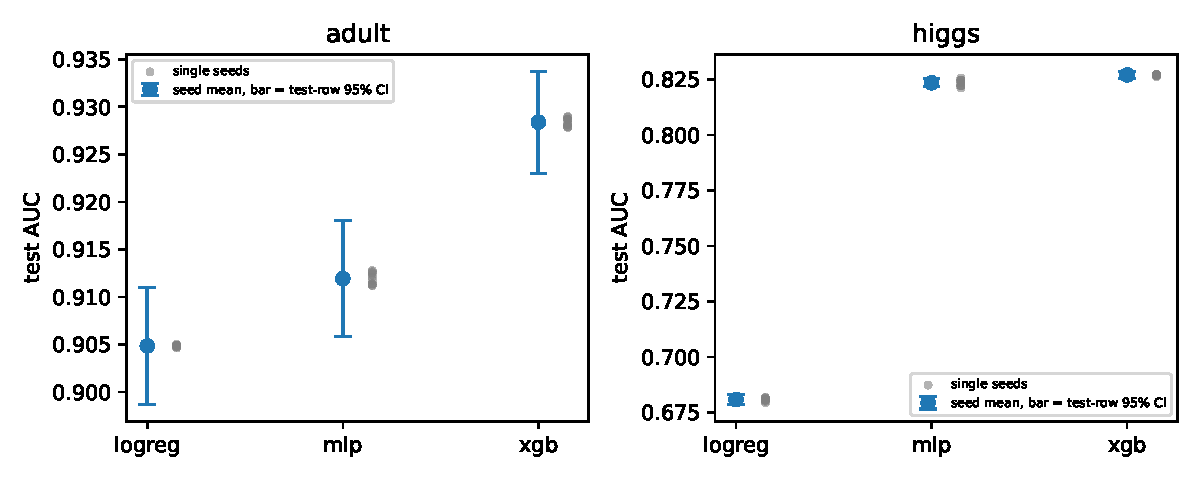
\includegraphics[width=0.92\textwidth]{accuracy.pdf}
\caption{Test AUC by model. Blue points are seed means with bars showing the 95\% bootstrap interval over test rows (seed 0 predictions); gray dots are the ten individual seeds. The third panel zooms in on the MLP and XGBoost on HIGGS.}
\label{fig:acc}
\end{figure*}

\textbf{Seed uncertainty against test-set uncertainty.} On Adult, the test-row half-width of the AUC (0.0054 to 0.0062) is about 10 to 60 times the seed standard deviation (0.0001 to 0.0006), because the test set has only 9{,}769 rows. Seed variation is almost negligible in comparison. On HIGGS, with 200{,}000 test rows, the half-width (0.0017 to 0.0023) is only 1.3 to 5.7 times the seed standard deviation (0.0003 to 0.0014), and for the MLP the two are comparable: the MLP is the least stable model across seeds, with AUC ranging from 0.8213 to 0.8256. XGBoost is the most stable model on both datasets.

\begin{table*}[t]
\caption{AUC differences between models (first minus second) with 95\% intervals. The seed bootstrap resamples each model's seeds independently and compares seed means. The row bootstrap is paired over test rows and uses seed 0 predictions. Every interval excludes zero.}
\label{tab:diff}
\centering
\begin{tabular}{llcc}
\toprule
Dataset & Comparison & Seed bootstrap & Row bootstrap (paired) \\
\midrule
Adult & Logistic regression $-$ MLP & $-0.0071$ [$-0.0075$, $-0.0067$] & $-0.0067$ [$-0.0089$, $-0.0045$] \\
Adult & Logistic regression $-$ XGBoost & $-0.0235$ [$-0.0238$, $-0.0233$] & $-0.0240$ [$-0.0270$, $-0.0211$] \\
Adult & MLP $-$ XGBoost & $-0.0164$ [$-0.0169$, $-0.0160$] & $-0.0173$ [$-0.0199$, $-0.0148$] \\
\midrule
HIGGS & Logistic regression $-$ MLP & $-0.1427$ [$-0.1436$, $-0.1418$] & $-0.1416$ [$-0.1438$, $-0.1394$] \\
HIGGS & Logistic regression $-$ XGBoost & $-0.1462$ [$-0.1467$, $-0.1458$] & $-0.1467$ [$-0.1488$, $-0.1446$] \\
HIGGS & MLP $-$ XGBoost & $-0.0035$ [$-0.0044$, $-0.0027$] & $-0.0051$ [$-0.0061$, $-0.0042$] \\
\bottomrule
\end{tabular}
\end{table*}

\textbf{Model differences.} Table~\ref{tab:diff} shows that all six pairwise differences exclude zero under both bootstraps. The smallest is the MLP versus XGBoost on HIGGS, which deserves care. Its two estimates differ (0.0035 from seed means, 0.0051 from seed 0), because seed 0 happens to be a below-average MLP seed (AUC 0.8223 against a mean of 0.8235), so the paired row estimate slightly overstates the typical gap. The MLP's seed range (0.0043) is larger than the gap itself, yet every XGBoost seed (minimum 0.8263) still exceeds every MLP seed (maximum 0.8256). The test-row bars in the third panel of Fig.~\ref{fig:acc} overlap, but that does not contradict the result: the paired comparison scores both models on the same rows, which removes most of the shared row-to-row noise and is much more sensitive than comparing two separate intervals. We therefore describe XGBoost's advantage on HIGGS as small but consistent.

\subsection{Computational cost}
Table~\ref{tab:cost} and Fig.~\ref{fig:cost} show the CPU cost of each model. XGBoost is the cheapest to train on Adult (1.20~s against 2.02~s for logistic regression and 6.90~s for the MLP) and also the most accurate. On HIGGS, XGBoost trains in 58.6~s, about four times faster than the MLP (240~s) and with a slightly higher AUC, so XGBoost beats the MLP on both accuracy and training time on both datasets. Logistic regression is cheapest on HIGGS (29.9~s) but about 0.146 AUC behind. Its training time here includes the shared PyTorch loop (batch size 256, early stopping), so it reflects that setup and not the intrinsic cost of a linear model.

Inference reverses the picture. Throughput falls from logistic regression (16 to 47M samples/s) to the MLP (1.1 to 2.0M) to XGBoost (0.28 to 0.63M), and the median latency of a single-row call is 0.12~ms, 0.28 to 0.29~ms and 0.75 to 0.88~ms respectively (p95 at most 1.34~ms). At batch size 1024 the median latency is 0.14 to 0.19~ms for logistic regression, 0.97 to 1.26~ms for the MLP and 2.5 to 5.6~ms for XGBoost. XGBoost is therefore the best trade-off for training but the slowest model to serve. Peak RSS ranges from 0.88 to 1.45~GB and is dominated by the loaded data and libraries, so we do not interpret differences between models.

\begin{table}[t]
\caption{CPU cost per model. Training time is the mean $\pm$ s.d.\ of three repeats; inference is the throughput on the full test set (millions of samples per second); latency is p50 / p95 for a batch of one row; RSS is the peak process memory.}
\label{tab:cost}
\centering
\footnotesize
\setlength{\tabcolsep}{3pt}
\begin{tabular}{llrrrr}
\toprule
Data & Model & Train (s) & Infer. & Lat. (ms) & RSS (MB) \\
\midrule
Adult & LogReg & $2.02 \pm 0.00$ & 16.2 & 0.12 / 0.16 & 880 \\
Adult & MLP    & $6.90 \pm 0.11$ & 1.14 & 0.29 / 0.34 & 1004 \\
Adult & XGB    & $1.20 \pm 0.01$ & 0.63 & 0.75 / 0.92 & 1005 \\
HIGGS & LogReg & $29.9 \pm 0.1$  & 47.2 & 0.12 / 0.16 & 996 \\
HIGGS & MLP    & $240 \pm 10$    & 2.04 & 0.28 / 0.34 & 1449 \\
HIGGS & XGB    & $58.6 \pm 0.5$  & 0.28 & 0.88 / 1.34 & 1028 \\
\bottomrule
\end{tabular}
\end{table}

\begin{figure*}[t]
\centering
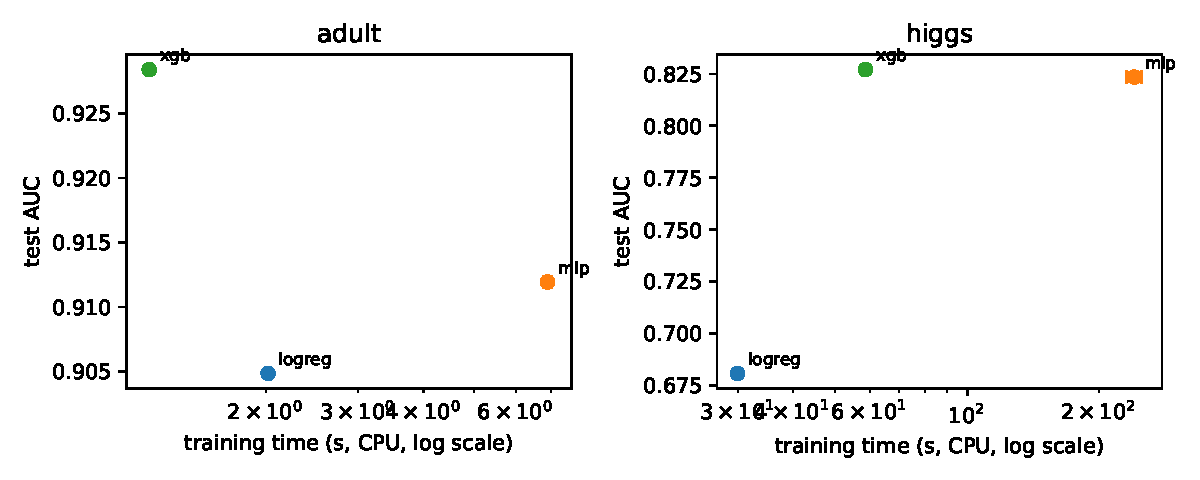
\includegraphics[width=0.7\textwidth]{cost_vs_accuracy.pdf}
\caption{Test AUC against CPU training time (log scale; horizontal bars show one standard deviation over three repeats).}
\label{fig:cost}
\end{figure*}

\textbf{Measurement conditions.} The cost runs were taken with the Windows ``Balanced'' power plan and about 19\% to 25\% background CPU load on the 12-thread machine (measured shortly afterwards), and the HIGGS fits were 2.0 to 2.6 times slower than the same fits during the earlier ten-seed runs (about 15, 106 and 22~s per seed for logistic regression, the MLP and XGBoost, including loading and tracking overhead). A single-repeat profiler run of the same logistic regression fit also gave 21.8~s against 29.9~s over three repeats, so process-to-process variation was large. Absolute times should therefore be read as indicative of one loaded laptop, and only large gaps, such as the MLP against XGBoost training time, should be treated as findings.

\subsection{Pandas against PySpark preprocessing}
\label{sec:spark}
This experiment runs on a Google Colab free-tier machine (2 CPU cores, 13.6~GB RAM, PySpark 4.0.5, OpenJDK~21~\cite{zaharia2016}). The pipeline reads the raw HIGGS CSV, drops null rows, standardizes the 28 features with the full-data mean and sample standard deviation, casts to 32-bit floats and writes Parquet. The Pandas version reads the CSV in one process. The Spark version runs in local mode with an explicit schema (no inference pass), one aggregation pass for the mean and standard deviation and one pass for the transformation and write. Each run is a separate subprocess; we report its wall-clock time (including interpreter or JVM startup) and the peak RSS of the whole process tree, sampled every 0.2~s. The datasets are the first 1M, 5M and all 11M rows of the file, and each setting was run once.

\begin{table}[t]
\caption{Preprocessing wall-clock time and peak memory (Colab free tier, 2 cores, one run per cell).}
\label{tab:spark}
\centering
\footnotesize
\setlength{\tabcolsep}{3pt}
\begin{tabular}{lrrrrr}
\toprule
Rows & Pandas (s) & Pandas (GB) & Spark (s) & Spark (GB) & Spark/Pandas \\
\midrule
1M  & 21.8  & 0.99  & 118.2 & 1.58 & 5.4 \\
5M  & 95.2  & 4.60  & 361.9 & 1.74 & 3.8 \\
11M & 206.1 & 10.08 & 735.4 & 1.76 & 3.6 \\
\bottomrule
\end{tabular}
\end{table}

\begin{figure*}[t]
\centering
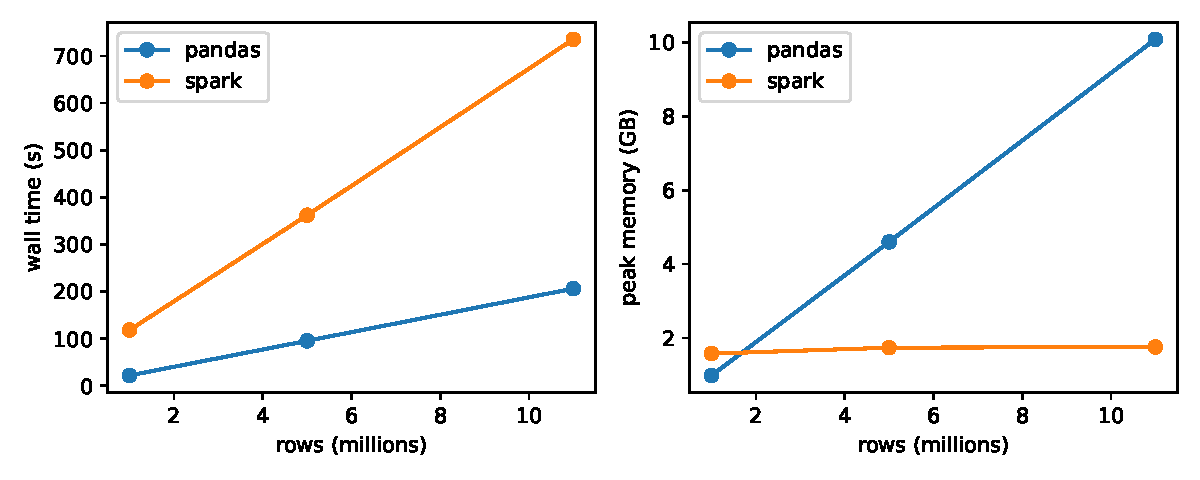
\includegraphics[width=0.7\textwidth]{spark_scaling.pdf}
\caption{Preprocessing wall-clock time (left) and peak memory (right) against the number of rows.}
\label{fig:spark}
\end{figure*}

Table~\ref{tab:spark} and Fig.~\ref{fig:spark} show that Pandas was faster at every size on this two-core machine, and that Spark's disadvantage shrank as the data grew (5.4 times at 1M rows, 3.6 times at 11M), as its fixed startup of about 16 to 18~s mattered less. Two cores leave little parallel work for Spark to exploit, so this result says little about a real cluster. Memory behaves differently: Pandas grows linearly to 10.1~GB at 11M rows (74\% of the machine's RAM), while Spark stays near 1.7 to 1.8~GB. At roughly 0.9~GB per million rows, linear growth would exhaust 13.6~GB at around 15M rows, although we did not test this. The partition count of Spark made no visible difference at 1M rows (112 to 135~s for 4, 8, 16 and 32 partitions, with peak memory 1.3 to 1.4~GB), within the noise of single runs.

File format mattered more than the engine (Table~\ref{tab:fmt}). Parsing the CSV took 77\% to 80\% of the Pandas pipeline time at every size. Reading the Parquet output was 15 to 24 times faster than reading the CSV, and the files were about 12 times smaller. This is a read-time comparison for this pipeline and not a controlled format benchmark: the Parquet files contain the standardized 32-bit output and were just written (warm cache), whereas the CSV is raw text parsed to 64-bit floats.

\begin{table}[t]
\caption{CSV against Parquet: file size and Pandas read time.}
\label{tab:fmt}
\centering
\footnotesize
\setlength{\tabcolsep}{3pt}
\begin{tabular}{lrrrrr}
\toprule
Rows & CSV (GB) & Parquet (GB) & CSV (s) & Parquet (s) & Speedup \\
\midrule
1M  & 0.73 & 0.06 & 16.4  & 1.1 & 15$\times$ \\
5M  & 3.65 & 0.31 & 72.0  & 3.0 & 24$\times$ \\
11M & 8.04 & 0.69 & 157.4 & 6.6 & 24$\times$ \\
\bottomrule
\end{tabular}
\end{table}

\section{Limitations}
\begin{itemize}
\item Ten seeds give only rough seed-based intervals, which tend to be too narrow, and the data split is fixed, so variation between splits is not measured.
\item The row bootstrap uses seed 0 predictions and conditions on one trained model. HIGGS uses 2{,}000 resamples instead of 10{,}000.
\item Hyperparameters are small, fixed and untuned, so the rankings describe these settings and not each model's best case. Both datasets use the same settings.
\item All timings are CPU only. Cost numbers come from one laptop under background load (Section~\ref{sec:cost}), and we do not report GPU results or the speed cost of deterministic mode.
\item The Spark benchmark runs once per setting on shared free-tier hardware with two cores, uses the first $N$ rows of the file, and polls memory every 0.2~s, so short peaks may be missed. It does not represent a multi-node cluster.
\item Logistic regression shares the MLP's training loop, so its training time is not that of a dedicated solver.
\end{itemize}

\section{Reproducibility}
The code, configurations, per-seed results, predictions and the Colab notebook are in a public repository.\footnote{\url{https://github.com/dishayayyy/mlbench}} After installing the package (\texttt{pip install -e ".[dev]"}), one Adult experiment runs with \texttt{python scripts/run\_experiment.py --config configs/adult\_logreg.yaml}, and seed 0 should give a logistic regression AUC of 0.9046 on the test set. The scripts for the cost runs, the two bootstraps and the tables and figures in this report are in the \texttt{scripts} folder, and the repository README lists the full command sequence.

\section{Conclusion}
Reporting both seed and test-set uncertainty changes how the results read. On Adult the test set is small enough that its sampling error dominates, while the ranking of the models is still robust. On HIGGS, training randomness of the MLP is as large as its test uncertainty, and XGBoost's lead over it is small but consistent. XGBoost gave the best accuracy and the shortest training time among the nonlinear models, but the slowest inference, so the preferable model depends on whether training or serving dominates. For preprocessing, the file format mattered more than the engine, and Pandas was both faster and, up to 11M rows, still feasible in memory on a 13.6~GB machine. The protocol and the caveats above are intended to make such comparisons easy to repeat and to qualify.

\begin{thebibliography}{99}
\bibitem{bouthillier2021} X. Bouthillier et al., ``Accounting for variance in machine learning benchmarks,'' in \emph{Proc. Machine Learning and Systems (MLSys)}, 2021.
\bibitem{dua2019} D. Dua and C. Graff, ``UCI Machine Learning Repository,'' University of California, Irvine, 2019. [Online]. Available: \url{https://archive.ics.uci.edu}
\bibitem{baldi2014} P. Baldi, P. Sadowski, and D. Whiteson, ``Searching for exotic particles in high-energy physics with deep learning,'' \emph{Nature Communications}, vol. 5, art. 4308, 2014.
\bibitem{chen2016} T. Chen and C. Guestrin, ``XGBoost: A scalable tree boosting system,'' in \emph{Proc. 22nd ACM SIGKDD Int. Conf. Knowledge Discovery and Data Mining}, 2016, pp. 785--794.
\bibitem{paszke2019} A. Paszke et al., ``PyTorch: An imperative style, high-performance deep learning library,'' in \emph{Advances in Neural Information Processing Systems 32}, 2019.
\bibitem{kingma2015} D. P. Kingma and J. Ba, ``Adam: A method for stochastic optimization,'' in \emph{Proc. Int. Conf. Learning Representations (ICLR)}, 2015.
\bibitem{zaharia2018} M. Zaharia et al., ``Accelerating the machine learning lifecycle with MLflow,'' \emph{IEEE Data Engineering Bulletin}, vol. 41, no. 4, pp. 39--45, 2018.
\bibitem{pedregosa2011} F. Pedregosa et al., ``Scikit-learn: Machine learning in Python,'' \emph{Journal of Machine Learning Research}, vol. 12, pp. 2825--2830, 2011.
\bibitem{efron1993} B. Efron and R. J. Tibshirani, \emph{An Introduction to the Bootstrap}. New York, NY, USA: Chapman \& Hall, 1993.
\bibitem{hanley1982} J. A. Hanley and B. J. McNeil, ``The meaning and use of the area under a receiver operating characteristic (ROC) curve,'' \emph{Radiology}, vol. 143, no. 1, pp. 29--36, 1982.
\bibitem{grinsztajn2022} L. Grinsztajn, E. Oyallon, and G. Varoquaux, ``Why do tree-based models still outperform deep learning on typical tabular data?'' in \emph{Advances in Neural Information Processing Systems 35, Datasets and Benchmarks Track}, 2022.
\bibitem{zaharia2016} M. Zaharia et al., ``Apache Spark: A unified engine for big data processing,'' \emph{Communications of the ACM}, vol. 59, no. 11, pp. 56--65, 2016.
\end{thebibliography}

\end{document}